\documentclass[draft]{beamer}
\usepackage{hyperref,xspace,graphicx,microtype,minted,multicol,mflogo}
\usepackage[brazil]{babel}

\usetheme[sectionpage=simple,numbering=none]{metropolis}
\beamertemplatenavigationsymbolsempty

\newcommand{\filename}[1]{\texttt{#1}}
\newcommand{\code}[1]{\texttt{#1}}

\title{Olá, \LaTeX!}
\author{Rafael Beraldo}
\date{28 de maio de 2016}

\begin{document}
\maketitle

\begin{frame}[standout]
  \Huge História e filosofia vão aqui
\end{frame}

% Considerações iniciais
\begin{frame}
  \only<1>{\Huge\LaTeX{} é uma linguagem de marcação de texto}
  \only<2>{\Huge Você \emph{declara} o documento}
  \only<3>{\Huge É como um tipógrafo profissional à sua disposição}
  \only<4>{\Huge Comandos são semânticos}
\end{frame}

% Sintaxe dos comandos
\begin{frame}[fragile]
  \begin{minted}[autogobble,fontsize=\huge,breaklines]{latex}
    \section{Introdução}
  \end{minted}
\end{frame}

% hello-world.tex %%%%%%%%%%%%%
\begin{frame}[standout]
  \huge
  \filename{hello-world.tex}
\end{frame}

\begin{frame}[fragile]
  \frametitle{\filename{hello-world.tex}}
  \begin{minted}[autogobble,fontsize=\Large,breaklines]{latex}
    \documentclass{article}
    \begin{document}
      Hello, world!
    \end{document}
  \end{minted}
\end{frame}

\begin{frame}[fragile]
  \frametitle{\filename{hello-world.tex}}
  \begin{minted}[autogobble,fontsize=\LARGE,breaklines]{bash}
    lualatex hello-world.tex
  \end{minted}
\end{frame}

\begin{frame}[fragile]
  \frametitle{\filename{hello-world.tex}}
  \begin{minted}[autogobble,breaklines]{latex}
    % hello-world.tex
    %
    % Rafael Beraldo <rberaldo@cabaladada.org>
    % Workshop de LaTeX do Opensanca
    % 28 de maio de 2016
  \end{minted}
\end{frame}

% Vamos cometer uns erros de propósito e lidar com as consequências?
\begin{frame}
  \frametitle{\filename{hello-world.tex}}
  \Huge
  Erros de compilação
\end{frame}

% espaco-branco.tex %%%%%%%%%%%%%%
% No exemplo, temos dois parágrafos do Guia do Mochileiro das Galáxias.
\begin{frame}[standout]
  \huge
  \filename{espaco-branco.tex}
\end{frame}

% Ensinar que, para criar uma nova linha, usamos estes comandos.
\begin{frame}[fragile]
  \frametitle{\filename{espaco-branco.tex}}
  \begin{minted}[autogobble,fontsize=\LARGE,breaklines]{latex}
    \\newline

    \\
  \end{minted}
\end{frame}

% Mostrar a extensão dos exercícios; pedir que o resolvam. Mostrar como os
% comentários contém as instruções.
\begin{frame}
  \frametitle{\filename{espaco-branco-exercicio.tex}}
  \LARGE
  Resolver \filename{espaco-branco-exercicio.tex}
\end{frame}

% poliglota-exercicio.tex %%%%%%%%%%%%%%
\begin{frame}[standout]
  \huge
  \filename{poliglota-exercicio.tex}
\end{frame}

% No exemplo anterior, espaco-branco.tex, os acentos --- na verdade,
% diacríticos --- não apareceram. Alguém saberia o motivo?
\begin{frame}
  \frametitle{\filename{poliglota-exercicio.tex}}
  \huge
  Acentos não apareciam em \filename{espaco-branco.tex}
\end{frame}

% Para resolver, teremos que usar pacotes
\begin{frame}
  \frametitle{\filename{poliglota-exercicio.tex}}
  \Huge
  Solução: pacotes
\end{frame}

% Para carregar pacotes, usamos esta sintaxe
\begin{frame}[fragile]
  \frametitle{\filename{poliglota-exercicio.tex}}
  \begin{minted}[autogobble,fontsize=\LARGE,breaklines]{latex}
    \usepackage[opções]{pacote}
  \end{minted}
\end{frame}

% Para resolvermos a falta de diacríticos, usaremos o pacote polyglossia
\begin{frame}
  \frametitle{\filename{poliglota-exercicio.tex}}
  \Huge
  Pacote \code{polyglossia}
\end{frame}

\begin{frame}
  \frametitle{\filename{poliglota-exercicio.tex}}
  \Huge
  O \code{polyglossia} traz benefícios como:
  \begin{itemize}
    \only<1>{\item Hifenização}
    \only<2>{\item Strings como \mintinline{latex}{\today}}
    \only<3>{\item Convenções tipográficas localizadas}
  \end{itemize}
\end{frame}

% Ao exercício.
%
% Sabemos para que serve o polyglossia. Perguntar como ele seria implementado,
% e onde seria colocado no código.
%
% Também estudar a sintaxe para selecionar línguas. Explicar o motivo pelo qual
% a opção de pacote [brazil] não é mais usada: fica difícil selecionar várias
% línguas e suas opções.
\begin{frame}
  \frametitle{\filename{poliglota-exercicio.tex}}
  \Huge
  Como carregar o pacote \code{polyglossia}?
\end{frame}

\begin{frame}[fragile]
  \frametitle{\filename{poliglota-exercicio.tex}}
  \begin{minted}[autogobble,fontsize=\Large,breaklines]{latex}
    \usepackage{polyglossia}
    \setdefaultlanguage{brazil}
  \end{minted}
\end{frame}

% Para encontrar ajuda, podemos ler a documentação oficial dos pacotes que
% estamos usando. Mostrar outras opções do polyglossia, por exemplo.
\begin{frame}
  \frametitle{\filename{poliglota-exercicio.tex}}
  \Huge
  Comprehensive \TeX{} Archive Network

  \url{ctan.org}
\end{frame}

\begin{frame}
  \frametitle{\filename{poliglota-exercicio.tex}}
  \huge
  \url{https://www.ctan.org/pkg/polyglossia}
\end{frame}

% artigo-exercicio.tex %%%%%%%%%%%%%%
\begin{frame}[standout]
  \huge
  \filename{artigo-exercicio.tex}
\end{frame}

% Dar uma olhada no arquivo. Ensinar a distinção entre o preâmbulo e o corpo do
% documento.
\begin{frame}
  \frametitle{\filename{artigo-exercicio.tex}}
  \LARGE
  Exemplo de arquivo comum em \LaTeX: \filename{artigo-exemplo.tex}
\end{frame}

% Explicar as opções da classe article que escolhi
\begin{frame}[fragile]
  \frametitle{\filename{artigo-exercicio.tex}}
  \huge
  Classes comuns:
  \begin{multicols}{2}
    \begin{itemize}
      \item\code{article}
      \item\code{report}
      \item\code{book}
      \item\code{letter}
      \item\code{memoir}
      \item\code{beamer}
  \end{itemize}
\end{multicols}
\end{frame}

% Vejamos quais são as opções de classe mais comuns
\begin{frame}
  \frametitle{\filename{poliglota-exercicio.tex}}
  \LARGE
  Opções de classe comuns:
  \begin{itemize}
    \only<1>{\item \code{10pt, 11pt, 12pt}}
    \only<1>{\item \code{a4paper, a5paper, letterpaper, …}}
    \only<1>{\item \code{fleqn}}
    \only<2>{\item \code{leqno}}
    \only<2>{\item \code{titlepage, notitlepage}}
    \only<2>{\item \code{twocolumn}}
    \only<2>{\item \code{twoside, oneside}}
    \only<3>{\item \code{landscape}}
    \only<3>{\item \code{openright, openany}}
    \only<3>{\item \code{draft}}
  \end{itemize}
\end{frame}

% Compilar o documento várias vezes, com opções diferentes
\begin{frame}
  \frametitle{\filename{poliglota-exercicio.tex}}
  \Huge
  Testar diferentes opções de classe
\end{frame}

% Olharemos agora os pacotes carregados
\begin{frame}
  \frametitle{\filename{poliglota-exercicio.tex}}
  \Huge
  Pacotes: \code{polyglossia, blindtext} e \code{hyperref}
\end{frame}

% Mudar o comando author para o seguinte
\begin{frame}[fragile]
  \frametitle{\filename{poliglota-exercicio.tex}}
  \LARGE
  Colocar um email abaixo dessa linha:
  \begin{minted}[autogobble,fontsize=\LARGE,breaklines]{latex}
   \author{Rafael Beraldo}
  \end{minted}
\end{frame}

\begin{frame}
  \frametitle{\filename{poliglota-exercicio.tex}}
  \Huge
  Adicionar o pacote \code{microtype}
\end{frame}

% Mostrar as diferenças entre usar ou não a protrusão e extensão de caracteres
\begin{frame}
  \frametitle{\filename{poliglota-exercicio.tex}}
  \LARGE
  Manual do \code{microtype}:\\
  \url{www.ctan.org/pkg/microtype}
\end{frame}

% O corpo do documento. O que são esses dois primeiros comandos?
\begin{frame}[fragile]
  \frametitle{\filename{poliglota-exercicio.tex}}
  \begin{minted}[autogobble,fontsize=\LARGE,breaklines]{latex}
  \begin{document}
  \frenchspacing
  \maketitle
  …
  \end{document}
  \end{minted}
\end{frame}

% \frenchspacing era utilizado no século 19, mas não mais
\begin{frame}
  \frametitle{\filename{poliglota-exercicio.tex}}
  \Large
  Exemplo de \mintinline{latex}{\frenchspacing}:

  \vspace{1em}
  \begin{minipage}{.45\textwidth}
    \nonfrenchspacing
    \mintinline{latex}{\nonfrenchspacing}:

    “A poesia vogon é, como todos sabem, a terceira pior do Universo. Em segundo
    lugar vem a poesia dos azgodos de Kria.”
  \end{minipage}
  \hspace{.05\textwidth}
  \begin{minipage}{.45\textwidth}
    \frenchspacing
    \mintinline{latex}{\frenchspacing}:
    
    “A poesia vogon é, como todos sabem, a terceira pior do Universo. Em segundo
    lugar vem a poesia dos azgodos de Kria.”
  \end{minipage}
\end{frame}

% Como organizar seu documento em seções
\begin{frame}
  \frametitle{\filename{poliglota-exercicio.tex}}
  \Large
  Comandos para seccionar o documento:

  \begin{itemize}
    \only<1>{\item \code{\textbackslash part}}
    \only<1>{\item \code{\textbackslash chapter}} (apenas classes \code{book} e
    \code{report})
    \only<1>{\item \code{\textbackslash section}}
    \only<1>{\item \code{\textbackslash subsection}}
    \only<1>{\item \code{\textbackslash subsubsection}}
    \only<1>{\item \code{\textbackslash paragraph}}
    \only<1>{\item \code{\textbackslash subparagraph}}
  \end{itemize}
\end{frame}

% Aquivos auxiliares
\begin{frame}[fragile]
  \frametitle{\filename{poliglota-exercicio.tex}}
  \LARGE
  Arquivos auxiliares:

  \begin{minted}[autogobble,fontsize=\Large,breaklines]{bash}
    artigo-exemplo.aux
    artigo-exemplo.log
    artigo-exemplo.out
    artigo-exemplo.pdf
    artigo-exemplo.tex
  \end{minted}
\end{frame}

% Para limpar aquivos auxiliares, uma das possibilidades é utilizar o latexmk
% com a opção -c (clean)
\begin{frame}
  \frametitle{\filename{poliglota-exercicio.tex}}
  \Huge
  Limpar arquivos auxiliares:

  \code{\$ latexmk -c}
\end{frame}

\begin{frame}
  \frametitle{\filename{poliglota-exercicio.tex}}
  \Huge
  Resolver \filename{poliglota-exercicio.tex}
\end{frame}

% fontes.tex %%%%%%%%%%%%%%
\begin{frame}[standout]
  \huge
  \filename{fontes.tex}
\end{frame}

% MetaFont era o sistema original, mas hoje usamos principalmente fontes do
% tipo OpenType
\begin{frame}
  \frametitle{\filename{fontes.tex}}
  \Huge
  \MF, Truetype (\code{ttf}) \& OpenType (\code{otf})
\end{frame}

% Na tabela ASCII, há apenas 95 caracteres imprimíveis. Nenhum deles é
% acentuado.
\begin{frame}[plain]
  \hspace*{-11.5mm}
  \begin{centering}
    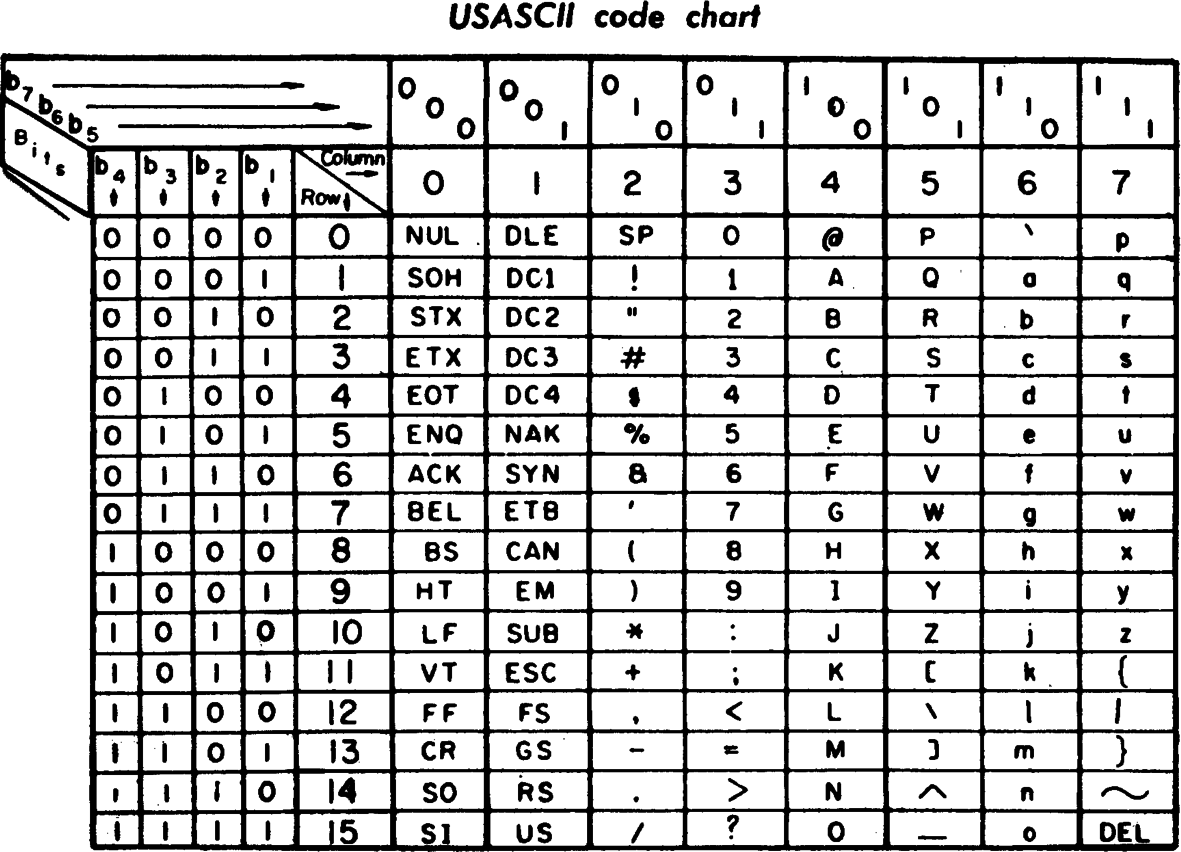
\includegraphics[width=\paperwidth]{images/ascii-chart}
    \par
  \end{centering}
\end{frame}

% A primeira codificação ficou conhecida como OT1 e a maior parte dos
% caracteres veio da tabela ASCII. Sintaxe para inserir acentos.
\begin{frame}[fragile]
  \frametitle{\filename{fontes.tex}}
  \huge
  \code{OT1}: Old Text 1
  \vspace{1em}

  \verb+Eur\'{i}pides+: Eur\'{i}pides
\end{frame}

% Essa abordagem tinha vários problemas.
\begin{frame}
  \frametitle{\filename{fontes.tex}}
  \huge
  Problemas da \code{OT1}:

  \begin{itemize}
    \only<1>{\item Palavras acentuadas não hifenizavam}
    \only<2>{\item Não era possível buscar por palavras acentuadas, muito menos
    copiá-las}
    \only<3>{\item E outros sistemas de escrita?}
  \end{itemize}
\end{frame}

% O problema começou a ser resolvido (para nós, falantes de português) mais de
% dez anos após o lançamento do LaTeX
\begin{frame}
  \frametitle{\filename{fontes.tex}}
  \huge
  1990 em Cork, Irlanda: nasce o \code{T1}, com 256 glifos
\end{frame}

% Quando comecei a usar LaTeX, aprendi a usar os seguintes pacotes e opções.
% Hoje, vamos aprender uma maneira melhor de fazer isso.
\begin{frame}[fragile]
  \frametitle{\filename{fontes.tex}}
  \begin{minted}[autogobble,fontsize=\LARGE,breaklines]{latex}
    \usepackage[utf8]{inputenc}
    \usepackage[T1]{fontenc}
  \end{minted}
\end{frame}

% Vamos falar sobre a diferença entre Unicode e os algorítimos de codificação
\begin{frame}
  \frametitle{\filename{fontes.tex}}
  \Huge
  \only<1>{Chega o Unicode!}
  \only<2>{Hoje com 120\,000 caracteres}
  \only<3>{Não é uma codificação, mas como uma tabela}
  \only<4>{UTF-8, UTF-16 e UTF-32 fazem o trabalho sujo}
  \only<5>{Hoje em \LaTeX, temos a codificação de fonte \code{TU}}
\end{frame}

% O pacote fontspec é carregado automaticamente pelo polyglossia, mas
% carregaremos ele mesmo assim.
\begin{frame}[fragile]
  \frametitle{\filename{fontes.tex}}
  \huge
  Aproveitar as vantagens do Unicode:

  \begin{minted}[autogobble,fontsize=\huge,breaklines]{latex}
    \usepackage{fontspec}
  \end{minted}
\end{frame}

% Exemplo do que podemos fazer usando LaTeX e Unicode. É claro, a fonte tem que
% conter os caracteres que estamos tentando usar.
\begin{frame}
  \frametitle{\filename{fontes.tex}}
  \Huge
  Εὐριπίδης — meu amigo de tantos anos — só lê Достое́вский.
\end{frame}

% Vamos aprender a acessar os diversos tipos de uma família de fontes. Vamos
% discutir com mais profundidade no exemplo e exercício.
\begin{frame}[fragile]
  \frametitle{\filename{fontes.tex}}
  \Huge
  \only<1>{Fontes vêm em famílias}
  \only<2>{\mintinline{latex}{\emph}: \emph{ênfase}}
  \only<3>{\mintinline{latex}{\textbf}: \textbf{negrito}}
  \only<4>{\mintinline{latex}{\textsc}: \textsc{Versaletes}}
  \only<5>{\mintinline{latex}{\texttt}: \texttt{teletipo}}
\end{frame}

% Tamanhos de fontes em LaTeX. Geralmente não é uma boa ideia usar eles à mão,
% pois os designers das classes de documento tomam essas decisões para nós. 
\begin{frame}[fragile]
  \frametitle{\filename{fontes.tex}}
  \large
  Tamanhos de fonte:
  \begin{multicols}{2}
    \begin{itemize}
      \item{\code{\textbackslash tiny}: 5pt}
      \item{\code{\textbackslash scriptsize}: 7pt}
      \item{\code{\textbackslash footnotesize}: 8pt}
      \item{\code{\textbackslash small}: 9pt}
      \item{\code{\textbackslash normalsize}: 10pt}
      \item{\code{\textbackslash large}: 12pt}
      \item{\code{\textbackslash Large}: 14pt}
      \item{\code{\textbackslash LARGE}: 17pt}
      \item{\code{\textbackslash huge}: 20pt}
      \item{\code{\textbackslash Huge}: 25pt}
    \end{itemize}
  \end{multicols}
\end{frame}

\begin{frame}
  \frametitle{\filename{fontes.tex}}
  \begin{quote}
    \underline{\textbf{Remember\Huge!}} \textit{The}
    \textsf{M\textbf{\LARGE O} \texttt{R}\textsl{E}} fonts \Huge you
    \tiny use \footnotesize \textbf{in} a \small \texttt{document},
    \large \textit{the} \normalsize more \textsc{readable} and
    \textsl{\textsf{beautiful} it bec\large o\Large m\LARGE e\huge s}.
  \end{quote}
\end{frame}

% Como trocar as fontes. Explicar que fontes matemáticas são outra história.
\begin{frame}[fragile]
  \frametitle{\filename{fontes.tex}}
  \Large
  Carregar fontes usando o \code{fontspec}:

  \begin{minted}[autogobble,fontsize=\Large,breaklines]{latex}
    \usepackage{fontspec}
      \setmainfont{Linux Libertine}
  \end{minted}
\end{frame}

% Fontes devem estar nos diretórios padrão. Caso não estejam, podemos
  % especificar um diret´orio:
\begin{frame}[fragile]
  \frametitle{\filename{fontes.tex}}
  \Large
  Especificar um diretório:

  \begin{minted}[autogobble,fontsize=\Large,breaklines]{latex}
    \usepackage{fontspec}
      \setmainfont{Linux Libertine}[
        Path = fonts/
      ]
  \end{minted}
\end{frame}

% Ligaduras são sequências de letras que naturalmente colidem. Por isso, são
% substituídas por outro caractere.
\begin{frame}
  \frametitle{\filename{fontes.tex}}
  \Huge
  Linux Libertine e ligaduras

  \fontspec{Linux Libertine}{
    affair\qquad fjord\qquad flor\\
    af\mbox{}fair\qquad f\mbox{}jord\qquad f\mbox{}lor
  }
\end{frame}

% Antes do exercício, vamos rever os conceitos que discutimos de maneira
% prática.
\begin{frame}
  \frametitle{\filename{fontes.tex}}
  \Huge
  Demonstrar ideias em \filename{fontes.tex}
\end{frame}

% Resolver o exercício fontes-exercicio.tex.
\begin{frame}
  \frametitle{\filename{fontes.tex}}
  \Huge
  Resolver \filename{fontes-exercicio.tex}
\end{frame}

% layouts-pagina.tex %%%%%%%%%%%%%%
\begin{frame}[standout]
  \Huge
   \filename{layouts-pagina.tex}
\end{frame}

% Vamos mudar a opção de classe de onecolumn para twocolumn e carregar o pacote
% showframe.
\begin{frame}
  \frametitle{\filename{layouts-pagina.tex}}
  \huge
  \only<1>{Copiar solução de \filename{fontes-exercio.tex} como
  \filename{layouts-pagina.tex}}
  \only<2>{Mudar para \code{twocolumn}, carregar o pacote \code{showframe}}
\end{frame}

% Na folha A4, apenas uma coluna coluna de texto é difícil de ler com margens
% curtas. Mas usar margens grandes desperdiça papel.
\begin{frame}
  \frametitle{\filename{layouts-pagina.tex}}
  \huge
  \code{onecolumn}: margens grandes demais

  \code{twocolumn}: nem sempre podemos
\end{frame}

% Soluções para o problema do tamanho da coluna de texto vs margens
\begin{frame}
  \frametitle{\filename{layouts-pagina.tex}}
  \huge
  Soluções:
  \begin{itemize}
    \only<1>{\item Colunas}
    \only<2>{\item \code{fullpage}}
    \only<3>{\item \code{fullpage} e entrelinhas maiores}
  \end{itemize}
\end{frame}

% Se decidirmos usar o pacote fullpage, é uma boa ideia aumentar o espaçamento
% entre as linhas.
\begin{frame}
  \frametitle{\filename{layouts-pagina.tex}}
  \huge
  Pacote \code{setspace}:

  \begin{itemize}
    \item \code{\textbackslash singlespacing}
    \item \code{\textbackslash onehalfspacing}
    \item \code{\textbackslash doublespacing}
  \end{itemize}
\end{frame}

% Outro fator que influencia o layout da página é seu estilo. Estes são os três
% comandos básicos e estilos que podemos escolher.
\begin{frame}
  \frametitle{\filename{layouts-pagina.tex}}
  \huge
  \code{\textbackslash pagestyle} e \code{\textbackslash thispagestyle}

  \begin{itemize}
    \item \code{empty}
    \item \code{plain}
    \item \code{headings}
  \end{itemize}
\end{frame}

% Outro fator que influencia o layout da página é seu estilo. Estes são os três
% comandos básicos e estilos que podemos escolher.
\begin{frame}
  \frametitle{\filename{layouts-pagina.tex}}
  \huge
  Demonstração em \filename{layouts-pagina.tex}
\end{frame}

% Faremos um certificado de conclusão do curso
\begin{frame}
  \frametitle{\filename{layouts-pagina.tex}}
  \Huge
  Certificado de conclusão
\end{frame}

% Uma ideia de como ele poderia ficar
\begin{frame}[plain]
  \begin{center}
    {\huge\textbf{OpenSanca}}\\[2em]
    {\LARGE\textsc{Certificado}}
  \end{center}

    \noindent Certificamos que Tal Pessoa da Silva participou de um curso em
    nosso grupo no dia 28 de maio de 2016 e está qualificado para editar textos
    em \LaTeX.

    \vfill
    \begin{flushright}
      \emph{Os Organizadores}\\
      \emph{OpenSanca}\\
    \end{flushright}
\end{frame}

% Começar nosso certificado de conclusão de curso
\begin{frame}
  \frametitle{\filename{layouts-pagina.tex}}
  \Huge
  Resolver \filename{layouts-pagina-exemplo.tex}
\end{frame}

% posicao-texto.tex %%%%%%%%%%%%%%
\begin{frame}[standout]
  \Huge
   \filename{posicao-texto.tex}
\end{frame}

% Nosso certificado pode ter ficado legal, mas poderia ser melhor ainda se
% ajustarmos o texto em relação à página.
\begin{frame}
  \frametitle{\filename{posicao-texto.tex}}
  \Huge
  Problemas com o certificado?
\end{frame}

% Antes de controlar a posição do texto, temos que entender o que é um
% ambiente.
\begin{frame}[fragile]
  \frametitle{\filename{posicao-texto.tex}}
  \Huge
  Ambientes:

  \begin{minted}[autogobble,fontsize=\Huge,breaklines]{latex}
    \begin{ambiente}
      …
    \end{ambiente}
  \end{minted}
\end{frame}

% Três ambientes para controlar posição.
\begin{frame}[fragile]
  \frametitle{\filename{posicao-texto.tex}}
  \Large
  Ambientes \code{center}, \code{flushleft} e \code{flushright}

  % Código:
  \begin{minted}[autogobble,fontsize=\Large,breaklines]{latex}
    \begin{center}
      Este texto será centralizado.
    \end{center}
  \end{minted}

  % Resultado:
  \begin{center}
    Este texto será centralizado.
  \end{center}
\end{frame}

% Ainda podemos controlar o espaço dentro de uma linha.
\begin{frame}[fragile]
  \frametitle{\filename{posicao-texto.tex}}
  \Huge
  \mintinline{latex}{\hspace{comprimento}}
\end{frame}

% Por exemplo, um espaço de 1,5cm:
\begin{frame}[fragile]
  \frametitle{\filename{posicao-texto.tex}}
  \LARGE
  \begin{minted}[autogobble,fontsize=\LARGE,breaklines]{latex}
    Essa frase\hspace{1.5cm} está esticada.
  \end{minted}
  \vspace{1em}

  Essa frase\hspace{1.5cm} está esticada.
\end{frame}

% O LaTeX aceita uma série de unidades
\begin{frame}[fragile]
  \frametitle{\filename{posicao-texto.tex}}
  \LARGE
  Unidades que o \LaTeX{} conhece:

  \begin{multicols}{2}
    \begin{itemize}
      \item\code{mm}
      \item\code{cm}
      \item\code{in}
      \item\code{pt}
      \item\code{em}
      \item\code{ex}
      \item\mintinline{latex}{\textheight}
      \item\mintinline{latex}{\textwidth}
      \item\mintinline{latex}{\pageheight}
      \item\mintinline{latex}{\pageheight}
    \end{itemize}
  \end{multicols}
\end{frame}

% O comando \hfill preenche todo o espaço disponível
\begin{frame}[fragile]
  \frametitle{\filename{posicao-texto.tex}}
  \LARGE
  \mintinline{latex}{Começo\hfill meio\hfill fim}
  \vspace{1em}

  Começo\hfill meio\hfill fim
\end{frame}

% E, finalmente, existem os comandos \vspace e \hfill
\begin{frame}[fragile]
  \frametitle{\filename{posicao-texto.tex}}
  \huge
  Comandos análogos:

  \mintinline{latex}{\vspace{comprimento}}
  \vspace{1em}

  \mintinline{latex}{\vfill}
\end{frame}
\end{document}
